% !TEX TS-program = pdflatex
% !TEX encoding = UTF-8 Unicode

% This file is a template using the "beamer" package to create slides for a talk or presentation
% - Giving a talk on some subject.
% - The talk is between 15min and 45min long.
% - Style is ornate.

% MODIFIED by Jonathan Kew, 2008-07-06
% The header comments and encoding in this file were modified for inclusion with TeXworks.
% The content is otherwise unchanged from the original distributed with the beamer package.

\documentclass{beamer}


% Copyright 2004 by Till Tantau <tantau@users.sourceforge.net>.
%
% In principle, this file can be redistributed and/or modified under
% the terms of the GNU General Public License, version 2.
%
% However, this file is supposed to be a template to be modified
% for your own needs. For this reason, if you use this file as a
% template and not specifically distribute it as part of a another
% package/program, I grant the extra permission to freely copy and
% modify this file as you see fit and even to delete this copyright
% notice. 


\mode<presentation>
{
  \usetheme{Warsaw}
  % or ...

  \setbeamercovered{transparent}
  % or whatever (possibly just delete it)
}


\usepackage[english]{babel}
% or whatever

\usepackage[utf8]{inputenc}
% or whatever

\usepackage{times}
\usepackage[T1]{fontenc}
% Or whatever. Note that the encoding and the font should match. If T1
% does not look nice, try deleting the line with the fontenc.

\usepackage{graphicx}
\graphicspath{ {../images/} }


\title{Pizza Knowledge Graph}

\author[Thomas Fishwick] % (optional, use only with lots of authors)
{T.~Fishwick\inst{1}}
% - Use the \inst{?} command only if the authors have different
%   affiliation.

\institute[Universities of Somewhere and Elsewhere] % (optional, but mostly needed)
{
  \inst{1}%
  City University}
% - Use the \inst command only if there are several affiliations.
% - Keep it simple, no one is interested in your street address.

\date[Short Occasion] % (optional)
{\today}

\subject{Talks}
% This is only inserted into the PDF information catalog. Can be left
% out. 



% If you have a file called "university-logo-filename.xxx", where xxx
% is a graphic format that can be processed by latex or pdflatex,
% resp., then you can add a logo as follows:

% \pgfdeclareimage[height=0.5cm]{university-logo}{university-logo-filename}
% \logo{\pgfuseimage{university-logo}}

% If you wish to uncover everything in a step-wise fashion, uncomment
% the following command: 

%\beamerdefaultoverlayspecification{<+->}


\begin{document}

\begin{frame}
  \titlepage
\end{frame}

\begin{frame}{Outline}
  \tableofcontents
\end{frame}


% Since this a solution template for a generic talk, very little can
% be said about how it should be structured. However, the talk length
% of between 15min and 45min and the theme suggest that you stick to
% the following rules:  

% - Exactly two or three sections (other than the summary).
% - At *most* three subsections per section.
% - Talk about 30s to 2min per frame. So there should be between about
%   15 and 30 frames, all told.

\section{Ontology Modelling}
%\subsection{Ontology Modelling}

\begin{frame}{Ontology Modelling}
	\begin{itemize}
		\item In my Knowledge Graph I have separated out the country, province, city, restaurant and menu items into different classes
		\item For the pizzas I have modelled various different types of pizza \& their ingredients
		\item Ingredient => Menu Item => Restaurant => City => State => Country
	\end{itemize}

\end{frame}

\section{Tabular Data to Knowledge Graph}
\begin{frame}{Tabular Data to Knowledge Graph}
	\begin{itemize}
		\item For getting the state \& country data no entity resolution was needed
		\item For the cities some more creativity was needed to match some of the cities up after the bulk of them were matched from the data from SPARQL queries to DBPedia
		\item To resolve the entities I built a map with words to look for in the menu name back to the ontology URL
	\end{itemize}
\end{frame}

\section{SPARQL \& Reasoning}
\subsection{Restaurants Selling Pizza Bianca}
\begin{frame}{Restaurants Selling Pizza Bianca}


\begin{center}
	Some of the restaurants serving Pizza Bianca
	\begin{tabular}{ | c | c | c | }
		\hline
		\textbf{Restaurant} & \textbf{City} & \textbf{State} \\
		\hline
		Planet Pizza & Greenwood Lake & New York \\
		\hline
		Nick's Pizza & Deerfield Beach & Florida \\
		\hline
		Caps Island Grille & Jensen Beach & Florida \\
		\hline
		Librettos Pizzeria & Charlotte & North Carolina \\
		\hline
		Mama's Pizza & Alpharetta & Georgia \\
		\hline
	\end{tabular}
\end{center}
\end{frame}

\subsection{SPARQL \& Reasoning}
\begin{frame}{SPARQL \& Reasoning}
	\begin{itemize}
		\item Average price of a Margherita pizza: \$12.05
		\item Number of restaurants: 2333
		\item Papa John's Pizza in Woodbury is the one missing its postcode
	\end{itemize}
\end{frame}

\section{Ontology Alignment}
\begin{frame}{Ontology Alignment}
	\begin{itemize}
		\item Originally there were several un-satisfiable classes, Ice Cream, Pizza Capricciosa, 4 Seasons and Siciliana
		\item For the 3 pizzas the issue was due to differences between their ingredients in the 2 ontologies
		\item For ice cream the problem was that in both ontologies the Has Topping property had the domain of pizza, by changing that to Food/Menu item in the ontologies this allowed it to be used
	\end{itemize}
\end{frame}

\section{Ontology Embeddings}
\subsection{Run OWL 2 Vec}
\begin{frame}{Run OWL 2 Vec}
	\begin{itemize}
		\item Here I used OWL 2 VEC to generate the embeddings for the ontology and the data.
		\item As there were characters in UTF-8 but not ASCII I had to modify the algorithm to use UTF-8 encodings.
		\item I tried using the reasoner and Weisfeiler-Leman walk, but these caused the algorithm to run for an indefinate amount of time.
	\end{itemize}
\end{frame}

\subsection{Vector Similarity}
\begin{frame}{Vector Similarity}
\begin{center}
	\begin{tabular}{ | c | c | c | c |}
		\hline
		\textbf{Words} & \textbf{Pizza Data} & \textbf{New Seed} & \textbf{Ontology} \\
		\hline
		pizza v tef:margherita & 0.198 & 0.183 & 0.297\\
		\hline
		margherita v tef:margherita & 0.349 & 0.266 & 0.482 \\
		\hline
		pizza v tef:pizza & 0.228 & 0.297 & 0.234 \\
		\hline
		american v tef:american & 0.312 & 0.257 & 0.427 \\
		\hline
		pizzaiola v tef:pizzaiola & 0.257 & 0.231 & 0.470 \\
		\hline
	\end{tabular}
\end{center}

\begin{itemize}
	\item The ontology model has higher similarities than the two data models.
	\item With the Margherita word against its concept having the highest score.
\end{itemize}
\end{frame}

\subsection{Clusters}
\begin{frame}{Clusters}
	\begin{itemize}
		\item Using PCA we can project the vectors into two components for the graph.
		\item PCA has split into three clusters.
		\item KMeans seems to look best with 8 clusters.
	\end{itemize}
	\center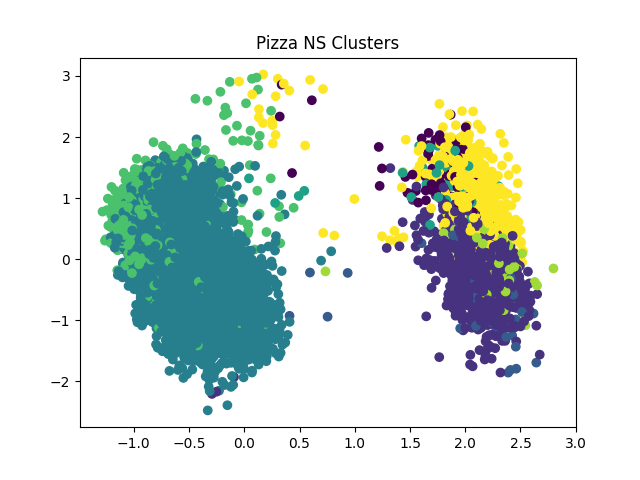
\includegraphics[scale=0.4]{pizzaDataModelClusters}
\end{frame}
\end{document}


